% Prepared by Calvin Kent
%
% Assignment Template v19.02
%
%%% 20xx0x/MATHxxx/Crowdmark/Ax
%
\documentclass[12pt]{article} %
\usepackage{CKpreamble}
\usepackage{CKassignment}
\usepackage{tkz-euclide}
\usepackage{physunits}
\usepackage{physics}
\usepackage{mathtools}
\usepackage{multicol}
\usepackage{lmodern}
\usepackage{tikz}
\usepackage{pgfplots}
\usepackage{pdfpages}
\usepackage{euscript}
\usepackage{transparent}
\usepackage{xcolor}
\usepackage{tasks}
\usepackage{tkz-euclide}

\usepackage{pgfplots}
\usepgfplotslibrary{polar}
\usepgflibrary{shapes.geometric}
\usetikzlibrary{calc}


\usepackage{euscript}
\usepackage{microtype}
\usepackage{upgreek}
\usepackage[misc]{ifsym}


%%Title
\title{\textbf{Assignment 3 Functions - SOLUTIONS} \\ \textbf{Due Date: } Tuesday, Feburary 1}
\date{}

%%% Maths and science packages

\usepackage{amsmath,amsthm,amssymb}
\usepackage{pgfplots}
	\usetikzlibrary{
		calc,
		patterns,
		positioning
	}
	\pgfplotsset{
		compat=1.16,
		samples=200,
		clip=false,
		my axis style/.style={
			axis x line=middle,
			axis y line=middle,
			legend pos=outer north east,
			axis line style={
				->,
			},
			legend style={
				font=\footnotesize
			},
			label style={
				font=\footnotesize
			},
			tick label style={
				font=\footnotesize
			},
			xlabel style={
				at={
					(ticklabel* cs:1)
				},
				anchor=west,
				font=\footnotesize,
			},
			ylabel style={
				at={
					(ticklabel* cs:1)
				},
				anchor=west,
				font=\footnotesize,
			},
			xlabel= $x$,
			ylabel=$\vec d (\m \tx{[East]})$
		},
	}
	\tikzset{
		>=stealth
	}

\pgfplotsset{my style/.append style={axis x line=middle, axis y line=
middle, xlabel={$t$}, ylabel={$y[\text{m}]$}, axis equal }}

%%% Tables and figures packages

\usepackage{float}
\usepackage{caption}
	\captionsetup{
		format=plain,
		labelfont=bf,
		font=small,
		justification=centering
	}
	
%%% Numbers and sets

\newcommand{\E}{\mathrm{e}}

\newcommand{\tx}[1]{\text{#1}}
\newcommand{\rem}[1]{\operatorname{rem}{(#1)}}


%
\begin{document}
	\pagenumbering{arabic}
	% Start of class settings ...
	\renewcommand*{\coursecode}{MATH 235} % renew course code
	\renewcommand*{\assgnnumber}{Assignment 1} % renew assignment number
	\renewcommand*{\submdate}{September 14, 2021} % renew the date
	\renewcommand*{\studentfname}{Abdullah} % Student first name
	\renewcommand*{\studentlname}{Zubair} % Student last name
    \renewcommand*{\proofname}{Proof:}
	% \renewcommand*{\studentnum}{20836288} % Student number

	\renewcommand\qedsymbol{$\blacksquare$}
	\setfigpath
	% End of class settings	
	% \pagestyle{crowdmark}
	\newgeometry{left=18mm, right=18mm, top=22mm, bottom=22mm} % page is set to default values
	\fancyhfoffset[L,O]{0pt} % header orientation fixed
	% End of class settings
	%%% Note to user:
	% CTRL + F <CHANGE ME:> (without the angular brackets) in CKpreamble to specify graphics paths accordingly.
	% The command \circled[]{} accepts one optional and one mandatory argument.
	% Optional argument is for the size of the circle and mandatory argument is for its contents.
	% \circled{A} produces circled A, with size drawn for letter A. \circled[TT]{A} produces circled A with size drawn for TT.
	% https://github.com/CalvinKent/My-LaTeX
	%%%

	%%%%%%%%%%%%%%%%%%%%%%%%%%%%%%%%%%%%%%%%%%%%%%%%%%%%%%%%%%%%%%%%%%%%%%%%%%%%%%%
	%%%                        CUSTOM MACRO VIM-TEX                             %%%
	%%       call IMAP('NOM', '\nomenclature{}', 'tex')               

	%%%%%%%%%%%%%%%%%%%%%%%%%%%%%%%%%%%%%%%%%%%%%%%%%%%%%%%%%%%%%%%%%%%%%%%%%%%%%%%

	% Crowdmark assignment start
	% qnumber, qname, qpoints
\maketitle
	\section{Preamble}
  This assignment covers everything taught so far. The solutions that you hand in should be \textbf{neat} and \textbf{legible},
  this is an assignment, not a quiz, so I expect you to take your time and present thorough and detailed solutions.

  This assignment has $\textbf{(REPLACE)}$ questions. \textbf{Start early}.
  \section{Replacement} 

  If your mark on this assignment is better than the last assignment, then I will replace the old assignment with
  this one. This means that your final assignment mark will consist of two assignment marks, either A1, A3 or A1,
  A2.

  \section{Bonus}
  If you type this assignment in \LaTeX, I will give you a bonus 7\%.
  
\section{Name and Date:}
	Print your name and todays date below;\\


	\begin{center}
	\noindent\begin{tabular}{ll}
		\makebox[3in]{\hrulefill} & \makebox[3in]{\hrulefill}\\
		Name & Date\\[8ex]% adds space between the two sets of signatures
	\end{tabular}
	\end{center}
	\newpage

  \begin{qstn}
    State in your own words, what does it mean for a number to be prime. What types of numbers can be primes? Why
    do we care about primes?
  \end{qstn}

  \begin{solution}
    A number $x$ is prime if its only positive divisors are $1$ and itself. Only natural numbers can be primes, and
    we care about as they are the building blocks for the fundamental theorem of arithmetic.
  \end{solution}

  \begin{qstn}
    Let $x \in \Z$ and let $p$ be a prime.
    \begin{enumerate}[label=(\alph*)]
      \item Determine all possible values of $\gcd (x,p)$.
        \begin{solution}
          Since $p$ is a prime, we have the following possible scenarios. Either $p$ divides $x$ perfectly, or it
          doesn't. In the former case, $\gcd (x,p) = p$, in the latter case, since the only other divisor of $p$ is
           $1$, we have that $\gcd(x,p) = 1$.
        \end{solution}
      \item Determine all possible values of $\gcd (x^2,p)$.
        \begin{solution}
          The key observation here is that nothing has really changed form part (a), we still have either of the
          two possibilities, either $p$ divides $x^2$ or it doesn't, $\gcd (x^2,p) = p$, in the former case and
          $\gcd (x^2,p) = 1$, in the latter case by similar reasoning from before.
        \end{solution}
      \item Determine all possible values of $\gcd (x,p^2)$.
        \begin{solution}
          In this case we have an additional scenario, either $p$ divides $x$, or $p^2$ divides $x$, or neither.
          By similar reasoning from before we conclude that the possible values for the gcd are, $\gcd(x,p^2) =
          p^2,p,1$. (The commas here mean the value can be this \textbf{or} this \textbf{or} this).
        \end{solution}
      \item Determine all possible values of $\gcd (x^2,p^2)$.
        \begin{solution}
          Again note that nothing has really changed from before, hence $\gcd(x^2,p^2) = p^2,p,1$.
        \end{solution}
      \item Determine all possible values of $\gcd (p^2,p)$.
        \begin{solution}
          Notice in this situation, there are no obscurities or ambiguities, albeit the state of $p$ is still
          arbitrary, you can convince yourself that regardless of the prime number we substitute, $p$ will
          \textbf{always} \textbf{divide} $p^2$. Hence
          $\gcd(p^2,p) = p$.
        \end{solution}
    \end{enumerate}
  \end{qstn}

  \begin{qstn}
    Let $p$ be a prime number. Determine the value of $ \operatorname{rem}(p,2)$ \textbf{and} explain how you got
    your answer.
    \begin{solution}
      The key observation here is that a prime number  $p$ \textbf{cannot} be an even number. Hence $p$ must be an
      odd number, from assignment $1$ we now that the remainder of an odd number divided by $2$ is $1$, and hence
      $\operatorname{rem}(p,2) = 1$.
    \end{solution}
  \end{qstn}

  \newpage
  
  \begin{qstn}
    This question is meant for review as it will definitely appear on the Final. Let $f(x) = \sqrt{x} $, 
    and let $R(x) = -2f(\frac{1}{2}x + 1) + 2$ be a transformation of $f$. 
    \begin{enumerate}[label=(\alph*)]
      \item Describe the transformation. \textbf{(Remember to Factor First)}
        \begin{solution}
          Let $A = -2, B = 1 / 2, H = 1, K = 2$.We first we factor $R(x)$ to obtain,
          \[
              R(x) = -2f\left(\frac{1}{2}x + 1\right)  + 2 = -2f\left( \frac{1}{2}(x + 2) \right) + 2
          .\] 
          From which we can describe the transformations,
          \begin{itemize}
            \item Since $A < 0$, $f$ is reflected across the x-axis.
            \item $f$ is horizontally shifted left by $2$ units.
            \item $f$ is vertically shifted up by $2$ units.
            \item Since $\left|A\right| = 2$ and $2 > 1$ we conclude that $f$ has been
              vertically stretched by a factor of $2$.
            \item  Since $ \left|B\right| = \frac{1}{2}$ and $0 < \frac{1}{2} < 1$ we conclude 
              that $f$ has been horizontally strethced by a factor  of $2$.
          \end{itemize}
        \end{solution}

      \item Determine the expression for the coordinate transformation,
        \[
          \left( \frac{x- H}{B}, Af(x) + K \right) =
          \left( 2(x - 1), -2f(x) + 2\right) 
        \] 

      \item Complete a coordinate table to determine the corresponding transformed coordinates using the following
        base coordinates,
        \[
            (0,0) \hspace*{2cm} (1,1) \hspace*{2cm} (4,2) \hspace*{2cm} (9,3) \hspace*{2cm} (16,4)
        .\] 
        \begin{solution} \texttt{  }
          \begin{center}
            \begin{tabular}{c|c}
          \text{$\left( x,f(x) \right) $} & \text{$ \left( 2(x - 1), -2f(x) + 2\right) $}\\\hline 
                \\
                $(0,0)$ & $(-2,2)$\\
                \\
                \\
                $(1,1)$ & $(0,0)$\\
                \\
                \\
                $(4,2)$ & $(6,-2)$\\
                \\
                \\
                $(9,3)$ & $(16,-4)$\\
                \\
                \\
                $(16,4)$ & $(30,-6)$\\
                \\
                \\
          \end{tabular}

          \end{center}
          
        \end{solution}


     \item Using your results from the coordinate table, sketch the transformation $R(x)$ \textbf{on your axis
       sheet}. Be sure to \textbf{label} the transformed coordinates as well as the function.

        \begin{center}
          
                  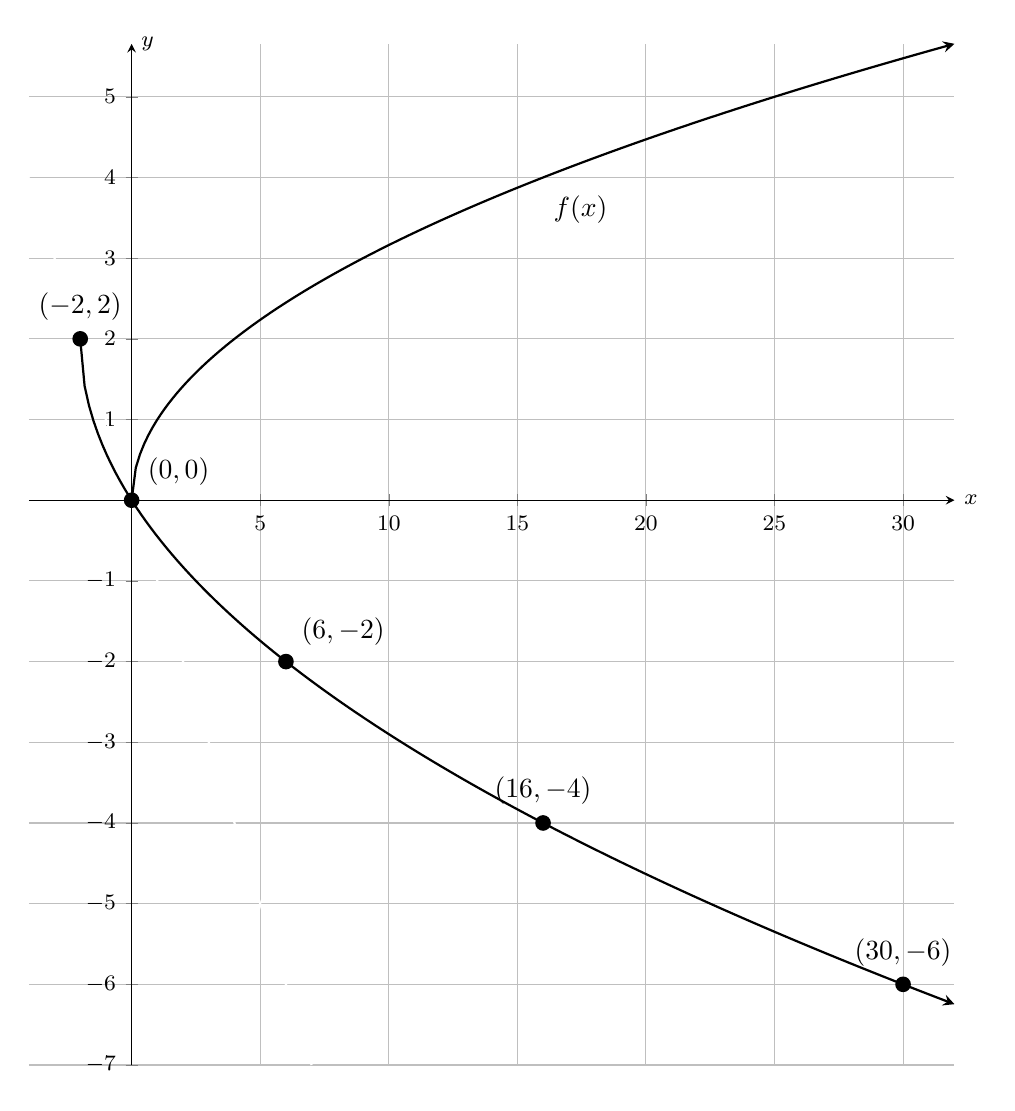
\begin{tikzpicture}
                  \begin{axis}[
                      my axis style,
                      width=1.1\textwidth,
                      height=1.2\textwidth,
                      ylabel=$y$,
                      grid
                  ]
                  
                  \addplot[
                      domain=-4:7,
                      thick,
                      white,
                      -
                  ]
                  {-x};
           
                  \addplot[
                      domain=0:32,
                      thick,
                      black,
                      ->
                  ]
                  {sqrt(x)};
                
                  \addplot[
                      domain=-2:32,
                      thick,
                      black,
                      ->
                  ]
                  {-2*sqrt(0.5*x + 1) + 2};


                  \fill[
                      black
                  ];

                  \node[label={275:{\textcolor{black}{$f(x)$}}},circle,inner sep=2pt] at (axis cs:16,4) {};

                  \node[label={90:{\textcolor{black}{$(-2,2)$}}},circle,fill,inner sep=2pt] at (axis cs:-2,2) {};
                  \node[label={40:{\textcolor{black}{$(0,0)$}}},circle,fill,inner sep=2pt] at (axis cs:0,0) {};
                  \node[label={45:{\textcolor{black}{$(6,-2)$}}},circle,fill,inner sep=2pt] at (axis cs:6,-2) {};
                  \node[label={90:{\textcolor{black}{$(16,-4)$}}},circle,fill,inner sep=2pt] at (axis cs:16,-4) {};
                  \node[label={90:{\textcolor{black}{$(30,-6)$}}},circle,fill,inner sep=2pt] at (axis cs:30,-6) {};

                  \end{axis}
                  \end{tikzpicture}
        \end{center}
    \end{enumerate}

  \end{qstn}

  \newpage

  \begin{qstn}
    Preform a prime factorization of the following natural numbers.\\
    \textbf{Note:} If the number is a prime itself, then state that it is.
    \begin{enumerate}[label=(\alph*)]
      \item 3634.
        \begin{solution}
          $3634 = 2 \cdot 23 \cdot  79$.
        \end{solution}
      \item 555.
        \begin{solution}
          $555 = 3 \cdot 5 \cdot 37$.
        \end{solution}
      \item 663.
        \begin{solution}
          $663 = 3 \cdot 13 \cdot 17$.
        \end{solution}
      \item 991.
        \begin{solution}
          $991$ is a prime number.
        \end{solution}
    \end{enumerate}
  \end{qstn}


  \begin{qstn}
    \textbf{Fully }simplify the following exponential expressions.\\ \textbf{(Leave answers with positive exponents)}
    \begin{enumerate}[label=(\alph*)]
      \item $-x^2(-x)^2x^{-3}$
        \begin{solution}
          $-x^2(-x)^2x^{-3} = -x$.
        \end{solution}
      \item $\left( x^{-4} \right) / \left( y^{2} \right)^{-3}  $.
        \begin{solution}
          \[
            \left( x^{-4} \right) / \left( y^{2} \right)^{-3} = \frac{y^{6}}{x^4}
          .\] 
        \end{solution}
      \item $\left( 4^{-1}y^2z^{-3}x^{8}x^{-3} \right)^{-3}y^{-6}z^{9}$.
        \begin{solution}
          \[
              \left( 4^{-1}y^2z^{-3}x^{8}x^{-3} \right)^{-3}y^{-6}z^{9} =
                      \frac{64z^{18}}{y^{12}x^{15}}
          .\] 
          
        \end{solution}
      \item $\left( 81a^{3}b^{2}z^{-6} \right)^{-2}  / \left( 3a^{9}bz^{-4} \right)^{-3}$.
        \begin{solution}
          \[
          \left( 81a^{3}b^{2}z^{-6} \right)^{-2}  / \left( 3a^{9}bz^{-4} \right)^{-3} = 
                \frac{a^{21}}{243b}
          .\] 
        \end{solution}
      \item $\left( 16 \right)^{\frac{3}{2}}\left( 9 \right)^{\frac{3}{2}} \left( 4\right) ^{\frac{-5}{2}} $.
        \begin{solution}
          \[
              \left( 16 \right)^{\frac{3}{2}}\left( 9 \right)^{\frac{3}{2}} \left( 4\right) ^{\frac{-5}{2}} =
                      54
          .\] 
        \end{solution}
    \end{enumerate}
  \end{qstn}

  \newpage
    
  \begin{qstn}
    \textbf{Textbook, Pg. 39\,\,\, Q1. a),c),e)}
  \end{qstn}

  \begin{qstn}
    \textbf{Textbook, Pg. 39\,\,\, Q3. a),c),e)}
  \end{qstn}

  \begin{qstn}
    \textbf{Textbook, Pg. 39\,\,\, Q4. a),c),e)}
  \end{qstn}

  \begin{qstn}
    \textbf{Textbook, Pg. 39\,\,\, Q5. a),c),e)}
  \end{qstn}
    
  \begin{qstn}
    \textbf{Textbook, Pg. 39\,\,\, Q7. a),c),e)}
  \end{qstn}

  \begin{qstn}
    \textbf{Textbook, Pg. 94\,\,\, Q4. a),c)}
  \end{qstn}

  \begin{qstn}
    \textbf{Textbook, Pg. 94\,\,\, Q6. c),d)}
  \end{qstn}

  \begin{qstn}
    \textbf{Textbook, Pg. 94\,\,\, Q6. b),c)}
  \end{qstn}
  \begin{solution}[Q7-Q14]
   \textbf{Refer to textbook solutions}
  \end{solution}

  \begin{qstn}
    You are given $\triangle SPQ$ where $SP = 13$,  $\angle PQS = 45^{\circ}$ and $\cos \beta = \sqrt{3} / 2$. Determine the
        \textbf{exact }area of  $\triangle SPQ$.
        \begin{center}
          \begin{tikzpicture}[thick]
          \coordinate (S) at (0,0);
          \coordinate (P) at (6,4);
          \coordinate (Q) at (15,0);
          \coordinate (R) at (6,0);

          \draw[black] (S) -- (Q) node[circle,fill,inner sep=2pt]{} node[above]{$Q$};
          \draw[black] (S) -- (P) node[circle,black,fill,inner sep=2pt]{} node[above]{$P$} node[midway, above]{$13$};
          \draw[black] (P) -- (Q) node[circle,black,fill,inner sep=2pt]{};
          \draw[dashed] (P) -- (R) node[circle,black,fill,inner sep=2pt]{};
          \draw[black] (S) node[circle,black,fill,inner sep=2pt]{} node[above]{$S$};
          \draw[black] (R) node[circle,black,fill,inner sep=2pt]{} node[below]{$R$};

          \tkzMarkAngle[fill= orange,size=1cm,%
          opacity=1](S,P,R)
          \tkzLabelAngle[pos = 1.4](S,P,R){$\beta$}

          \tkzMarkAngle[fill= orange,size=1.4cm,%
          opacity=1](P,Q,S)
          \tkzLabelAngle[pos = 1.8](P,Q,S){$45^{\circ}$}

          \tkzMarkRightAngle[size=0.4,opacity=0.9](S,R,P)% square angle here

          \end{tikzpicture}
      \end{center}
  \end{qstn}
  \begin{solution}
    \[
        A_{\triangle SPQ} = \frac{169}{8} \left( 3 + \sqrt{3}\right)
    .\] 
  \end{solution}

  \begin{qstn}
    Describe in your own words what polar coordinates are? Why are they useful and what advantages do they provide
    as a metric?
  \end{qstn}
  \begin{solution}
    Polar coordinates are a metric that parametrize euclidean space. They are useful because they provide an
    efficient and concise notation to describe coordinates, they are beneficial because they are isometries,
    or so called distance preserving metrics.
  \end{solution}

    \newpage

  \begin{qstn}
    Convert (a), (b) to polar coordinates and (c), (d) to standard coordinates.
    \begin{multicols}{4}
      \begin{enumerate}[label=(\alph*)]
        \item $\vb P(-3,4)$.
          \columnbreak
        \item $\vb R(-1,-3)$.
          \columnbreak
        \item $\vb Q(4,320 ^{\circ})$.
          \columnbreak
        \item $\vb T(9,30^{\circ})$.
      \end{enumerate}
      
    \end{multicols}


  \begin{solution} \texttt{  }
    \begin{enumerate}[label=(\alph*)]
      \item $\vb P(-3,4) = \vb P(5, 306.87^{\circ})$.
      \item $\vb R(-1,-3) = \vb P\left( \sqrt{10}, 251.565^{\circ}\right)$.
      \item $\vb Q(4,320^{\circ}) = \vb Q(3.064, -2.571)$.
      \item $\vb T(9,30^{\circ}) = \vb T\left( \frac{9\sqrt{3}}{2}, \frac{9}{2}\right)$.
    \end{enumerate}
  \end{solution}

  \end{qstn}

  \begin{qstn}
    Determine the six trigonometric ratios for the following angles,
    \begin{multicols}{4}
      \begin{enumerate}[label=(\alph*)]
        \item $\theta_1 = 60^{\circ}$
          \columnbreak
        \item $\theta_2 = 220^{\circ}$
          \columnbreak
        \item $\theta_3 = -240^{\circ}$
          \columnbreak
        \item $\theta_4 = 330^{\circ}$
      \end{enumerate}
      
    \end{multicols}
    \begin{solution} \texttt{  }
      \begin{enumerate}[label=(\alph*)]
        \item 
        \[
            \sin 60^{\circ} = \frac{\sqrt{3}}{2} \hspace{0.7cm} \cos 60^{\circ} = \frac{1}{2} \hspace{0.7cm} 
            \tan 60^{\circ} = \sqrt{3} 
        \] 

        \[
            \csc 60^{\circ} = \frac{2}{\sqrt{3}} \hspace{0.7cm} \sec 60^{\circ} = 2 \hspace{0.7cm} 
            \cot 60^{\circ} = \frac{1}{\sqrt{3}} 
        \] 
      \item 
        \[
            \sin 220^{\circ} = -0.642787 \hspace{0.7cm} \cos 220^{\circ} = -0.76604 \hspace{0.7cm} 
            \tan 220^{\circ} = -0.8390 
        \] 

        \[
            \csc 220^{\circ} = -1.55572 \hspace{0.7cm} \sec 220^{\circ} = -1.3054 \hspace{0.7cm} 
            \cot 220^{\circ} = 1.1917 
        \] 
    \item 
        \[
            \sin 240^{\circ} = -\frac{\sqrt{3}}{2} \hspace{0.7cm} \cos 240^{\circ} = -\frac{1}{2} \hspace{0.7cm} 
            \tan 240^{\circ} = \sqrt{3}.  
        \] 

        \[
            \csc 240^{\circ} = -\frac{2}{\sqrt{3}} \hspace{0.7cm} \sec 240^{\circ} = -2 \hspace{0.7cm} 
            \cot 240^{\circ} = \frac{1}{\sqrt{3}}.  
        \] 

    \item 
      \[
          \sin 330^{\circ} = -\frac{1}{2} \hspace{0.7cm} \cos 330^{\circ} = \frac{\sqrt{3}}{2}\hspace{0.7cm} 
          \tan 330^{\circ} = -\frac{1}{\sqrt{3}}.  
      \] 

      \[
          \csc 330^{\circ} = -2 \hspace{0.7cm} \sec 330^{\circ} =  \frac{2}{\sqrt{3}}  \hspace{0.7cm} 
          \cot 330^{\circ} = -\sqrt{3} .  
      \] 


      \end{enumerate}
      
    \end{solution}

  \end{qstn}













\end{document}



































